%!TEX root = main.tex
\change{\section{Evaluation Study Methods\label{sec:userstudy}}}
%between-subject
In this section, we describe the methodology 
for \change{a user study} 
we conducted for evaluating the 
\change{usefulness of \system 
for various exploratory analysis tasks.
We aim to evaluate whether \system
obeys the ``3S'' design principles in order
to effortlessly identify insights in comparison 
with other dashboard generation baselines.}
% addressing the following research questions:
% \begin{denselist}
% 	\item RQ1: How \textit{interesting} are the visualizations in the dashboard perceived subjectively by the users?
% 	\item RQ2: How well \change{does} the dashboard \textit{summarize} the relative importance of different attributes within a given dataset?
% 	\item RQ3: How \textit{informative} are the visualizations in the dashboard at providing users with an accurate understanding of unseen child visualizations?
% \end{denselist}
% These research questions roughly correspond to the three S's in our objective---saliency, summarization, and safety.

\subsection{\change{Participants and Conditions}}
We recruited 18 participants \change{(10 Male; 8 Female)}
with prior experience in working with data. 
Participants included undergraduate 
and graduate students, researchers, 
and data scientists, with 1 to 14 years of data 
analysis experience (average = 5.61). 
\tr{This can include, but are not limited to, browsing and reading data, data cleaning and wrangling, data visualization and model building. The inclusion criteria is assessed based on a self-reporting basis in the pre-study survey.} 
No participants reported prior experience 
in working with the two datasets used in the study (described below). 
Participants were randomly assigned two 
of the three types of dashboards with \change{$k=10$} 
visualizations generated \change{via the} 
following conditions. 
\papertext{\change{The specific dashboards for each dataset and condition are 
shown in our technical report for reference}.\agp{add citation}}
%(described in Section \ref{sec:algorithms})
\stitle{\system:} The dashboards for this condition 
are generated by the aforementioned 
frontier greedy algorithm and displayed 
in a hierarchical layout (as in Figure~\ref{fig:overview}). 
\tr{To ensure the informativeness of the generated dashboards, 
we selected a more stringent $\theta$=90\% 
criteria to generate the dashboards for our user study.} 
To establish a fair comparison 
with the two other conditions, 
we deactivated \tr{iceberg pruning (by setting $\delta$=0) and} 
the interactive node expansion capabilities.
\stitle{\BFS (short for breadth-first search):} 
Starting from the visualization of the \change{overall} population, 
$k$ visualizations are selected level-wise, 
traversing down the subset lattice, 
adding the visualizations at the first level 
with $1$-filter combination one at a time, 
\change{and then visualizations with $2$-filter combinations}, 
and so on, 
until $k$ visualizations have been added to the dashboard. 
This baseline is designed to simulate a dashboard 
generated by a meticulous analyst who exhaustively 
inspects all visualizations (i.e., filter combinations) 
from the top down. 
The chosen visualizations are displayed 
in a $5\times2$ table in the traversed order.
\stitle{\cluster:} \change{In this condition,}
$k$-Means clustering is first performed on the data distributions 
\change{of all of the visualizations in the lattice}. 
This results in $k$ clusters \change{that cover the rest of the}
visualizations. 
\change{For each cluster, we select
the visualization with the least number of filter conditions
as the cluster representative for interpretability}\tr{\footnote{Since the clusters cover all visualizations in the dataset and the overall visualization has the minimum number of filter across all visualization, the overall visualization is guaranteed to be picked as one of the displayed visualizations.}} 
and display them in a $5\times2$ table layout. 
This baseline is designed to showcase a diverse set of 
distributions within the dataset.
\tr{
  \begin{figure*}[ht!]
  \centering
  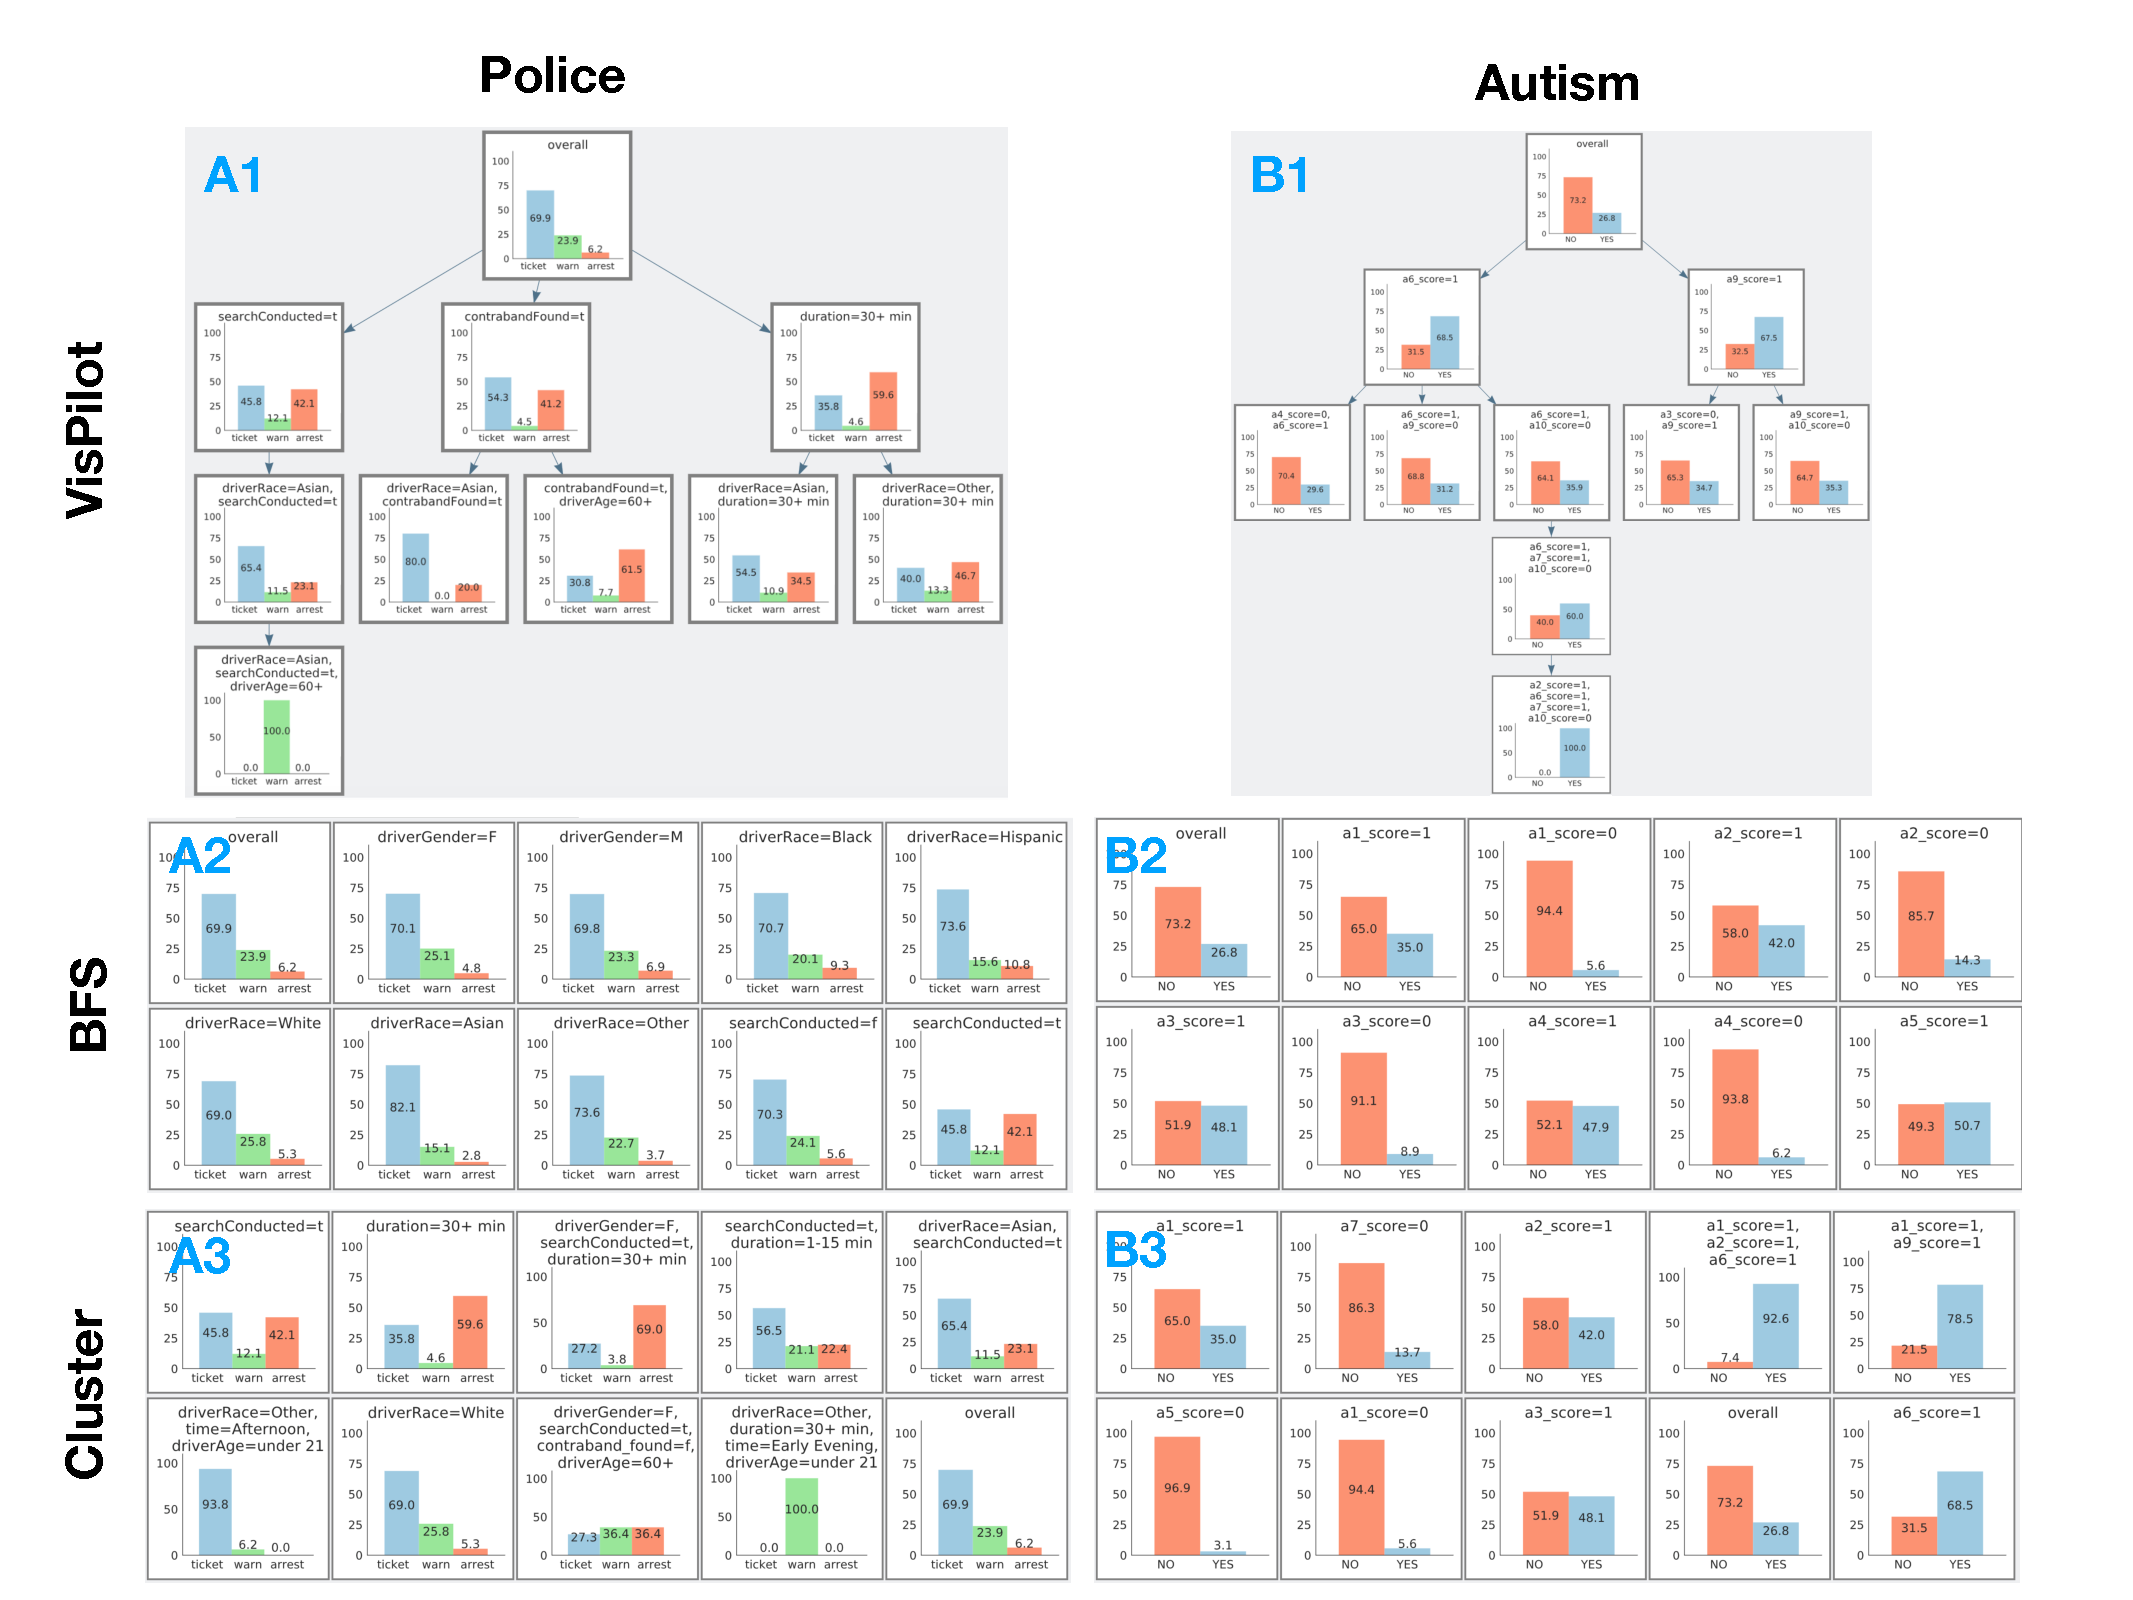
\includegraphics[width=0.95\linewidth]{figures/dashboard_examples.pdf}
  \caption{Specific dashboards for each dataset and condition used in the study.}
  \label{fig:dashboards}
  \vspace{-10pt}
  \end{figure*}
}
\smallskip
\stitle{Dataset Descriptions.} 
Each participant was assigned two different 
conditions on two different datasets 
\change{(Police Stop and Autism, described below)}. 
The ordering of each condition was 
randomized to prevent confounding learning effects. 
The study began with a 5-minute tutorial 
using dashboards generated from the Titanic dataset~\cite{titanic} 
for each condition. 
To prevent bias across conditions, 
participants were not provided an explanation of 
how the dashboards were generated and 
why the visualizations were arranged in a particular way. 

\change{The first dataset in the study} was the aforementioned 
Police Stop dataset. 
The attributes in the dataset 
include driver gender, age, race, stop time of day, 
stop outcome, whether a search was conducted, 
and whether contraband was found. 
We generated dashboards of bar chart visualizations 
with x-axis as the stop outcome 
(i.e., whether the police stop resulted in a 
ticket, warning, or arrest) and y-axis as the percentage of police stops that led to each outcome. %We randomize the ordering for each task combination to prevent confounding learning effects. %%, which contains visualizations of the \% of police stop that resulted in a warning, ticket, or an arrest. %, which contains a total of 312948 records of vehicle and pedestrian stops from law enforcement departments in Connecticut, dated from 2013 to 2015.

The second dataset in the study 
was the Autism dataset~\cite{autism}, 
\change{describing} the results of autism spectrum 
disorder screening for 704 adults. 
The attributes in the dataset are binary responses 
to 10 diagnostic questions 
as part of the screening process. 
This dataset serves as a data-agnostic condition, 
since there was no descriptions 
of the questions or answer labels provided to the 
\change{participants}. 
We generated dashboard visualizations 
based on whether the participant is diagnosed with autism or not.\agp{??????}

\change{\subsection{Study Procedure}
After the tutorial, for each dataset, participants}
were given some time to read through a worksheet 
containing the descriptions of the data attributes. 
Then, they were given an attention check question 
where they were 
\change{provided} 
a verbal description of the visualization filter 
\change{(i.e., data subset)}
and asked about the corresponding visualization in the dashboard. 
After understanding the dataset and chart schema, 
participants were asked to accomplish the following 
tasks in \change{the order listed}:
\stitle{\change{Interestingness Label (Saliency)}:} 
Participants were asked to talk aloud 
as they interpreted the visualizations 
in the dashboard and \change{label} 
each visualization as interesting or 
not interesting, \change{or leave it unselected}. 
This \change{subjective task measures} 
how \change{\emph{interesting} 
the selected visualizations were} 
to participants (RQ1).%well are participants at retrieving interesting visualizations (RQ1).
\stitle{Attribute Ranking \change{(Succinctness)}:} 
Participants were given a sheet of paper 
with all the attributes listed 
and asked to rank the attributes 
in order of importance in contributing 
to a particular outcome (e.g., factors leading to an arrest or autism diagnosis). Participants were allowed to assign equal ranks to more than one attribute or skip attributes that they were unable to infer importance for. 
Attribute ranking tasks are common in feature selection and other data science tasks.
\change{Since all dashboards were equally {\em compact} in
that they contained $k = 10$ visualizations, our goal was
to check whether this compactness came at the cost of {\em overall understanding}.
Thus, the goal of this task was to measure how well participants}
understood the relative importance of each attribute in contributing towards an outcome (RQ2).
\stitle{Informative Prediction \change{(Safety}):} 
Participants were given a separate worksheet 
and asked to sketch an estimate for a visualization 
that is not present in the dashboard. 
For every condition, the visualization to be estimated 
contained $2$ filter combinations, 
with exactly one parent present in the given dashboard. 
After making the prediction, 
participants were shown the actual data 
distribution and asked to rate on a Likert scale 
of 10 how surprising the result was 
\change{(1: not surprising and 10: very surprising)}. 
\change{This} task measured how accurate participants 
are at predicting an unseen visualization, 
estimating how well they understood key \emph{informative} insights that influences other distributions from the dataset (RQ3)\agp{I don't understand this RQ.}.

\smallskip
\noindent At the end of the study, we asked two open-ended questions regarding the insights 
\change{gained by} participants 
and what they 
\change{liked or disliked} 
about each dashboard. On average, the study lasted around 48 minutes.

\agp{Order of RQs here and in study results are different. The way the RQs are described are different as well. Please fix before I look at S5}
